\documentclass[12pt]{article}
\usepackage[noindent]{rajeev}
\setlength{\headheight}{14.49998pt}
\usepackage{graphicx}
\usepackage{listings}
\usepackage{amsmath}
\usepackage{amssymb}
\usepackage{geometry}
\geometry{a4paper, margin=1in}
\usepackage{color}


\begin{document}


\begin{center}
    \Large
    \sffamily 
    \textbf{Intro to AI Assignment 3 - Probabilistic Reasoning}

    \vspace{0.5cm}

    \large
    {Rajeev Atla -
    2008003072\\}
    
    {Dhvani Patel -
    210006030\\}
    
    {Jasmin Badyal -
    2008003131\\}

    \vspace{0.5cm}

    \today
\end{center}

\section{Problem 1}

\subsection{Part a}

The joint probability for the events $A, B, C, D, E$ 
is defined by the chain rule as:
$$P(A, B, C, D, E) = P(A) \cdot P(B) \cdot P(C) \cdot P(D|A, B) \cdot P(E|B, C)$$

For the specific case where all events are true ($T$), 
the joint probability is:
\begin{align*}
    P(A=T, B=T, C=T, D=T, E=T) &= P(A=T) \cdot P(B=T) \cdot P(C=T) \\
    & \cdot P(D=T|A=T, B=T) \cdot P(E=T|B=T, C=T)
\end{align*}

Substituting the provided numerical values:
\begin{align*}
P(A=T, B=T, C=T, D=T, E=T) &= 0.2 \cdot 0.5 \cdot 0.8 \cdot 0.1 \cdot 0.3 \\
&= 0.0024
\end{align*}

Thus, 
the likelihood of the combined event where 
$A, B, C, D$ and $E$ are all true is $\boxed{0.0024}$.

\subsection{Part b}

Now, 
let's analyze the scenario where all these events are false ($F$). 
The joint probability is:

\begin{align*}
P(A=F, B=F, C=F, D=F, E=F) &= P(A=F) \cdot P(B=F) \cdot P(C=F) \\
& \cdot  P(D=F|A=F, B=F) \cdot P(E=F|B=F, C=F) \\
\end{align*}

Inserting the given probabilities for this scenario:

\begin{align*}
P(A=F, B=F, C=F, D=F, E=F) &= 0.8 \cdot 0.5 \cdot 0.2 \cdot 0.1 \cdot 0.8 \\
&= 0.0064
\end{align*}

Consequently, 
the probability of the joint event where $A, B, C, D,$ 
and $E$ are all false is $\boxed{0.0064}$.

\subsection{Part c}

We aim to determine the conditional probability 
$P(\neg A | B, C, D, E)$. 
Employing Bayes' theorem, 
this can be expressed as proportional to the joint probability 
$P(\neg A, B, C, D, E)$:

$$P(\neg A | B, C, D, E) \propto P(\neg A, B, C, D, E).$$

Let the normalization factor be $\alpha$, 
defined as:

$$\alpha = \frac{1}{P(A, B, C, D, E) + P(\neg A, B, C, D, E)}.$$

We are given the calculation for $\alpha$:

$$\alpha = \frac{1}{(0.2 \cdot 0.5 \cdot 0.8 \cdot 0.1 \cdot 0.3) + (0.8 \cdot 0.5 \cdot 0.8 \cdot 0.6 \cdot 0.3)}.$$
$$\alpha = \frac{1}{0.0024 + 0.0576} = \frac{1}{0.06} = \frac{50}{3}.$$

Now, we can compute the conditional probability $P(\neg A | B, C, D, E)$:

$$P(\neg A | B, C, D, E) = \alpha \cdot P(\neg A, B, C, D, E).$$
$$P(\neg A | B, C, D, E) = \frac{50}{3} \cdot 0.0576.$$
$$P(\neg A | B, C, D, E) = 0.96.$$

Therefore, 
the conditional probability $P(\neg A | B, C, D, E)$ is $\boxed{0.96}$.

\section{Problem 2}

\subsection{Part a}

Our goal is to determine the conditional probability 
$P(\text{Burglary} | \text{JohnsCalls} = \text{true}, \text{MaryCalls} = \text{true})$. 
We are given the formulation:

$$P(B|J, M) = \alpha \cdot P(B) \sum_{E} P(E) \sum_{A} P(A|B, E) \cdot P(J|A) \cdot P(M|A)$$
where 
$\alpha = \frac{1}{P(J, M)}$.

Following the provided steps and correcting the final calculation:
\begin{align*}
P(B|J,M)
& = \alpha \cdot \begin{pmatrix} 0.00059224259 \\ 0.0014918576 \end{pmatrix} \\
& \left( \text{where the top element corresponds to } B=T \text{ and the bottom to } B=F \right) \\
& \left( \text{and } \alpha = \frac{1}{0.0020853609} \right) \\
& = \frac{1}{0.0020853609} \cdot \begin{pmatrix} 0.00059224259 \\ 0.0014918576 \end{pmatrix} \\
& = \begin{pmatrix} \frac{0.00059224259}{0.0020853609} \\ \frac{0.0014918576}{0.0020853609} \end{pmatrix} \\
& = \begin{pmatrix} 0.284 \\ 0.716 \end{pmatrix}
\end{align*}

Here, 
$\boxed{0.284}$ signifies the probability of a burglary occurring given that John and Mary call, 
while $\boxed{0.716}$ represents the probability of no burglary under the same conditions.

\subsection{Part b}

What is the computational cost of determining 
$P(X_1 | X_n = \text{true})$ 
via enumeration? 
What is the cost using variable elimination?

\subsubsection{Complexity via Enumeration}

To compute 
$P(X_1 | X_n = \text{true})$ 
by enumeration, 
we initially assess two binary trees for each state of $X_1$. 
Each of these trees possesses a depth of $n - 2$. 
Consequently, 
the aggregate computational effort for enumeration amounts to $\boxed{O(2^n)}$.

\subsubsection{Complexity via Variable Elimination}

Moving on to variable elimination, 
the size of the factors will not exceed two variables. 
For instance, 
when computing $P(X_1 | X_n = \text{true})$:

\begin{align*}
P(X_1 | X_n = \text{true})
& = \alpha \cdot P(X_1) \cdots \sum_{x_{n-2}} P(x_{n-2} | x_{n-3}) \sum_{x_{n-1}} P(x_{n-1} | x_{n-2}) P(X_n = \text{true} | x_{n-1}) \\
& = \alpha \cdot P(X_1) \cdots \sum_{x_{n-2}} P(x_{n-2} | x_{n-3}) \sum_{x_{n-1}} f_{X_{n-1}}(x_{n-1}, x_{n-2}) f_{X_n}(x_{n-1}) \\
& = \alpha \cdot P(X_1) \cdots \sum_{x_{n-2}} P(x_{n-2} | x_{n-3}) f_{\frac{x_{n-2}}{X_{n-1} \cdot X_n}}
\end{align*}

As evident, 
this mirrors a problem with $n-1$ variables rather than $n$. 
Hence, 
the computational work remains constant, 
independent of $n$, 
and the overall complexity is $\boxed{O(n)}$.


\section{Problem 3}

\subsection{Part A}

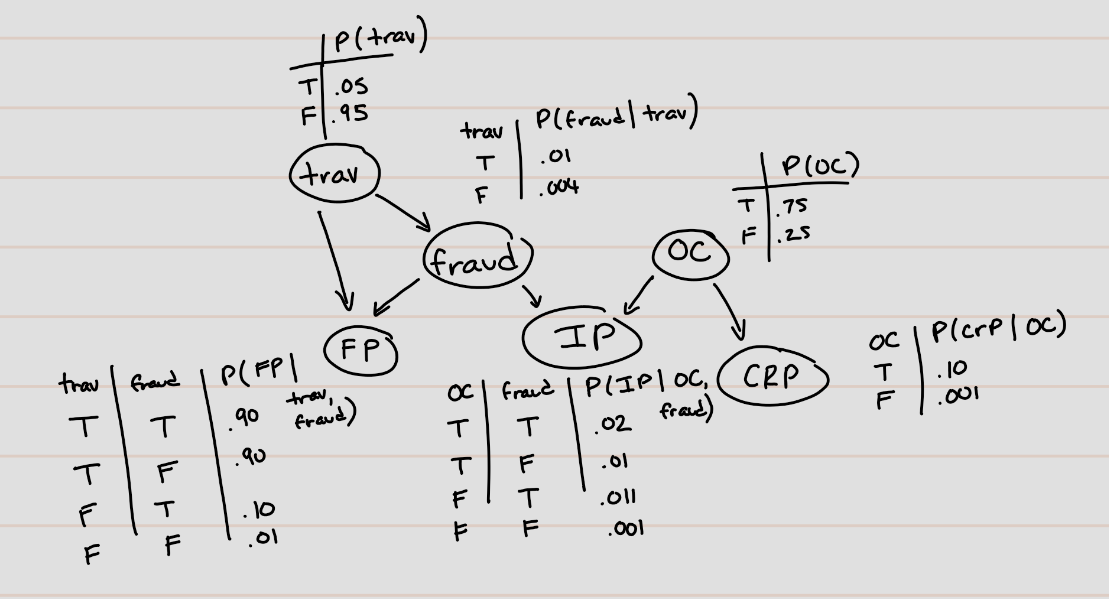
\includegraphics[scale=0.5, keepaspectratio]{part3a.png}

\subsection{Part B}

Prior probability of fraud:

$P(fraud) = P(travel) * P(fraud | travel) + P(\neg travel) * P(fraud | \neg travel)$

$ = 0.5 * P(fraud | travel) + 0.95 * P(fraud | \neg travel)$

$ = 0.5 * 0.01 + 0.95 * 0.004$

$ = 0.0088$

\space

$P(fraud | FP, \neg IP, CRP)$:


$P(fraud | FP, \neg IP, CRP) = α * P(fraud, FP, \neg IP, CRP)$

\space

$ P(fraud, FP, \neg IP, CRP) = \sum_{trav} \alpha \sum_{OC} P(trav) * P(fraud | trav) * P(FP | fraud, trav) * P(OC) * P(\neg IP | OC, fraud) * P(CRP | OC)$

$ = \sum_{OC} P(trav) * P(fraud | trav) * P(FP | fraud, trav) * P(OC) * P(\neg IP | OC, fraud) * P(CRP | OC) +

\sum_{OC} P(\neg trav) * P(fraud | \neg trav) * P(FP | fraud, \neg trav) * P(OC) * P(\neg IP | OC, fraud) * P(CRP | OC)$

$ = P(trav) * P(fraud | trav) * P(FP | fraud, trav) * P(OC) * P(\neg IP | OC, fraud) * P(CRP | OC) +

P(trav) * P(fraud | trav) * P(FP | fraud, trav) * P(\neg OC) * P(\neg IP | \neg OC, fraud) * P(CRP | \neg OC) +

P(\neg trav) * P(fraud | \neg trav) * P(FP | fraud, \neg trav) * P(OC) * P(\neg IP | OC, fraud) * P(CRP | OC) +

P(\neg trav) * P(fraud | \neg trav) * P(FP | fraud, \neg trav) * P(\neg OC) * P(\neg IP | \neg OC, fraud) * P(CRP | \neg OC)$

$ = 0.05 * 0.01 * .90 * .75 * (1 - 0.02) * 0.10 +

0.05 * 0.01 * .90 * .25 * (1 - 0.011) * 0.001 +

0.95 * 0.004 * .10 * .75 * (1 - 0.02) * 0.10 +

0.95 * 0.004 * .10 * .25 * (1 - 0.011) * 0.001$

$ = 0.000033075 + 1.112625\times10^{-7} + 0.00002793 + 9.3955\times10^{-8}$

$ = 0.0000612102175$

Next, calculate alpha. We first need $P(\neg fraud, FP, \neg IP, CRP)$.

$ P(\neg fraud, FP, \neg IP, CRP) = \sum_{trav} \alpha \sum_{OC} P(trav) * P(\neg fraud | trav) * P(FP | \neg fraud, trav) * P(OC) * P(\neg IP | OC, \neg fraud) * P(CRP | OC)$

$ = \sum_{OC} P(trav) * P(\neg fraud | trav) * P(FP | \neg fraud, trav) * P(OC) * P(\neg IP | OC, \neg fraud) * P(CRP | OC) +

\sum_{OC} P(\neg trav) * P(\neg fraud | \neg trav) * P(FP | \neg fraud, \neg trav) * P(OC) * P(\neg IP | OC, \neg fraud) * P(CRP | OC)$

$ = P(trav) * P(\neg fraud | trav) * P(FP | \neg fraud, trav) * P(OC) * P(\neg IP | OC, \neg fraud) * P(CRP | OC) +

P(trav) * P(\neg fraud | trav) * P(FP | \neg fraud, trav) * P(\neg OC) * P(\neg IP | \neg OC, \neg fraud) * P(CRP | \neg OC) +

P(\neg trav) * P(\neg fraud | \neg trav) * P(FP | \neg fraud, \neg trav) * P(OC) * P(\neg IP | OC, \neg fraud) * P(CRP | OC) +

P(\neg trav) * P(\neg fraud | \neg trav) * P(FP | \neg fraud, \neg trav) * P(\neg OC) * P(\neg IP | \neg OC, \neg fraud) * P(CRP | \neg OC)$

Alpha $= 1/(P(fraud, FP, \neg IP, CRP) + P(\neg fraud, FP, \neg IP, CRP))$.

The final answer is $0.0000612102175 * $ alpha

\section{Problem 4}

We can model the system as a hidden Markov model.
We can model $X_t$ as a Markov chain with the states 
$\set{A, B, C, D, E, F}$ 
and transition matrix:

\begin{align*}
    T_{i, j} &= P(X_t = j| X_{t-1} = i) \\
    T &= 
    \begin{pmatrix}
        0.2 & 0.8 & 0 & 0 & 0 & 0 \\
        0 & 0.2 & 0.8 & 0 & 0 & 0 \\
        0 & 0 & 0.2 & 0.8 & 0 & 0 \\
        0 & 0 & 0 & 0.2 & 0.8 & 0 \\
        0 & 0 & 0 & 0 & 0.2 & 0.8 \\
        0 & 0 & 0 & 0 & 0 & 1 \\
    \end{pmatrix}
\end{align*}

In addition,
we have the observation matrices for hot and cold:

\begin{align*}
    O_{\text{hot}} &= 
    \begin{pmatrix}
        1 & 0 & 0 & 0 & 0 & 0 \\
        0 & 0 & 0 & 0 & 0 & 0 \\
        0 & 0 & 0 & 0 & 0 & 0 \\
        0 & 0 & 0 & 1 & 0 & 0 \\
        0 & 0 & 0 & 0 & 0 & 0 \\
        0 & 0 & 0 & 0 & 0 & 0 \\
    \end{pmatrix} \\
    O_{\text{cold}} &= 
    \begin{pmatrix}
        0 & 0 & 0 & 0 & 0 & 0 \\
        0 & 1 & 0 & 0 & 0 & 0 \\
        0 & 0 & 1 & 0 & 0 & 0 \\
        0 & 0 & 0 & 0 & 0 & 0 \\
        0 & 0 & 0 & 0 & 1 & 0 \\
        0 & 0 & 0 & 0 & 0 & 1 \\
    \end{pmatrix} \\
\end{align*}

We know that the rover starts at state A with probability 1,
so $P(X_1 = A) = 1$.
The initial state vector is therefore $f_1 = [1, 0, 0, 0, 0, 0]^T$.

\subsection{Part 1}

We are being asked to compute the state distribution
$f_3$
given the observations 
$O_1 = \text{hot}$, $O_2 = \text{cold}$, and $O_3 = \text{cold}$.


\begin{align*}
    f_3 &= \alpha O_{e_3} T f_2 \\
    &= \alpha O_{e_3} T \pars{\alpha O_{e_2} T f_1} \\
    &= \alpha O_{\text{cold}} T  O_{\text{cold}} T f_1 \\
    &= \alpha 
    \begin{pmatrix}
        0 & 0 & 0 & 0 & 0 & 0 \\
        0 & 1 & 0 & 0 & 0 & 0 \\
        0 & 0 & 1 & 0 & 0 & 0 \\
        0 & 0 & 0 & 0 & 0 & 0 \\
        0 & 0 & 0 & 0 & 1 & 0 \\
        0 & 0 & 0 & 0 & 0 & 1 \\
    \end{pmatrix}
    \begin{pmatrix}
        0.2 & 0.8 & 0 & 0 & 0 & 0 \\
        0 & 0.2 & 0.8 & 0 & 0 & 0 \\
        0 & 0 & 0.2 & 0.8 & 0 & 0 \\
        0 & 0 & 0 & 0.2 & 0.8 & 0 \\
        0 & 0 & 0 & 0 & 0.2 & 0.8 \\
        0 & 0 & 0 & 0 & 0 & 1 \\
    \end{pmatrix} \\
    & \cdot
    \begin{pmatrix}
        0 & 0 & 0 & 0 & 0 & 0 \\
        0 & 1 & 0 & 0 & 0 & 0 \\
        0 & 0 & 1 & 0 & 0 & 0 \\
        0 & 0 & 0 & 0 & 0 & 0 \\
        0 & 0 & 0 & 0 & 1 & 0 \\
        0 & 0 & 0 & 0 & 0 & 1 \\
    \end{pmatrix}
    \begin{pmatrix}
        0.2 & 0.8 & 0 & 0 & 0 & 0 \\
        0 & 0.2 & 0.8 & 0 & 0 & 0 \\
        0 & 0 & 0.2 & 0.8 & 0 & 0 \\
        0 & 0 & 0 & 0.2 & 0.8 & 0 \\
        0 & 0 & 0 & 0 & 0.2 & 0.8 \\
        0 & 0 & 0 & 0 & 0 & 1 \\
    \end{pmatrix}
    \begin{pmatrix}
        1 \\
        0 \\
        0 \\
        0 \\
        0 \\
        0 \\
    \end{pmatrix} \\
    &= [0, 0.2, 0.8, 0, 0, 0] \\
\end{align*}




\section{Problem 5}

\end{document}
